\chapter{Estructura cristalina} \label{Ch:01}

Las sustancias cristalinas se caracterizan por una periodicidad espacial perfecta, que facilita enormemente la tarea de comprender y calcular sus propiedades físicas. Las sustancias cristalinas se encuentran comúnmente en forma de policristales (aglomerados de pequeñas cristales orientados desordenadamente llamadas cristalitos o granos). Existe una categoría importante de sólidos, que no se tratará aquí denominados amorfos, como el vidrio común  y muchos polímeros, que no pertenecen a los sólidos cristalinos, pues aunque poseen cierto orden de corto alcance carecen del orden de largo alcance característico de los cristales.

\section{Conceptos básicos}

En esta sección introduciremos las definiciones más importantes que usaremos a lo largo del tema. Es importante memorizarlos bien, ya que serán usados recursivamente a lo largo del libro. También es importante leerlos en el orden que proponemos, ya que muchos derivan de conceptos previos. Estas definiciones son fundamentales para el estudio de la Física del Estado Sólido, y dado que existe una amplísima gama de definiciones que podemos encontrar en la literatura, trataremos de incluir aquellas más interesantes. Dado que nuestro principal libro de referencia es el Física del Estado Sólido \cite{Fisica_del_Estado_Solido}, usaremos estas para definir los conceptos básicos, aunque es probable que introduzcamos cambios con la finalidad de que se entiendan mejor.


\subsection{Red}

El concepto de red es un concepto fundamental, por lo que es necesario tener muy claro su significado. 

\begin{definition}[\textbf{Red}]
	Una red es un conjunto de puntos discretos del espacio con vectores posición dados por la combinación lineal
	
	\begin{equation}
	\rn = u_1 \an_1 + u_2 \an_2 + u_3 \an_3 \label{Ec:01-01-01} 
	\end{equation}

	donde los $u_i$ barren todos los enteros. Los $\an_i$ se denominan \textbf{vectores bases primitivos}, y deben ser linealemente independientes.\label{Def:01-01}
\end{definition}

Con esto podremos tener una idea de lo que es una red. La red más básica que nos podemos imaginar en 2D es el conjunto de puntos definidos por los vectores $\hni$ y $\hnj$, mientras que en 3D es el conjunto de puntos formado por los vectores $\hni,\hnj$ y $\hnk$. Es bueno imaginarse un conjunto formado por otros vectores, como $\parentesis{\hni,\frac{1}{\sqrt{2}} (\hni +\hnj),\hnk}$, o $\parentesis{\hni,\frac{1}{\sqrt{2}} (\hni +\hnk),\hnk}$, ya que nos permitirá pensar rápidamente en varias redes. Como bien dice el Kittle \cite{Estado_Solido_Kittel}:  una red no es más que una distribución regular de puntos en el espacio, una abstracción matemática: para crear una estructura cristalina hace falta colocar átomos, y asignar estos a los puntos de la red. \\

Sin embargo la definición \ref{Def:01-01} es, en cierto modo, engañosa, ya que nos da a entender que si los puntos $u_i$ no son enteros no se puede formar una red, y esto es falso. Se puede formar una red con valores de $\an_1,\an_2$ y $\an_3$ con valores no enteros (por ejemplo, semienteros), solo que en este caso los vectores $\an_i$ serán \textit{\textbf{vectores no primitivos}}. Una definición muy interesante es la que dan en el capítulo 12 del \cite{Oxford_Solid_State}:

\begin{definition_equivalente}
	Una red es un conjunto de puntos donde el alrededor de cada uno de los puntos es indistinguible de cualquier otro punto. Véase la imagen \ref{Fig:01-00}
\end{definition_equivalente}

\begin{figure}[h!] \centering
	\includegraphics[scale=0.3]{Cuerpo/Ch_01/red.png}
	\caption{Como se puede ver $R$ y $P$ no son equivalentes, mientras que $P$ y $Q$ sí.}
	\label{Fig:01-00}
\end{figure}


\subsection{Base atómica y estructura cristalinas}

Como hemos mencionado en el párrafo anterior, para obtener un cristal tenemos que colocar átomos/moléculas en la red. Básicamente tenemos que asignar a cada punto de red una conjunto de átomos. A esto se le llamará base atómica, tal y como se define en \cite{Fisica_del_Estado_Solido}:

\begin{definition}[{\bf Base atómica}]
    Conjunto de átomos que se asocia a todos y cada uno de los puntos de la red. Se puede tener una base monoátomica (a cada punto de la red se le asocia un átomo), diatómica (dos átomos), triatómica (tres átomos)...
    \label{Def:01-Base_atomica}
\end{definition}

Una vez tenemos una red y una base atómica asociada a cada punto de red obtendremos la estructura cristalina:

\begin{definition}[{\bf Estructura cristalina o cristal}]
    Es la combinación red+base atómica, asociándose a cada punto de red una base atómica. 
\end{definition}

Aunque en el manual \cite{Fisica_del_Estado_Solido} no lo menciona, hay que diferenciar entre los vectores base primitivos de la estructura y cristal y vectores base primitivos de la red. Lógicamente podemos coger una base atómica de un número de átomos arbitrario. y hacer traslaciones sencillas para obtener la red cristalina. Sin embargo 

\subsection{Celda: celda unitaria, primitiva, Wigner-Seitz.}

Una celda es siempre un volumen o un área (en función de la dimensión del espacio), mientras que los diferentes adjetivos denotan las características para cada celda. El tipo de celda más importante es el tipo la celda unitaria primitva.

\begin{definition}[\textbf{Celda unitaria}]
	Volumen (en el caso de una red tridimensional, superficie en una red 2-dimensional) en el que encontramos un único punto de red, que mediante traslaciones puede recrear la red. 
\end{definition}


\begin{figure}[h!] \centering
	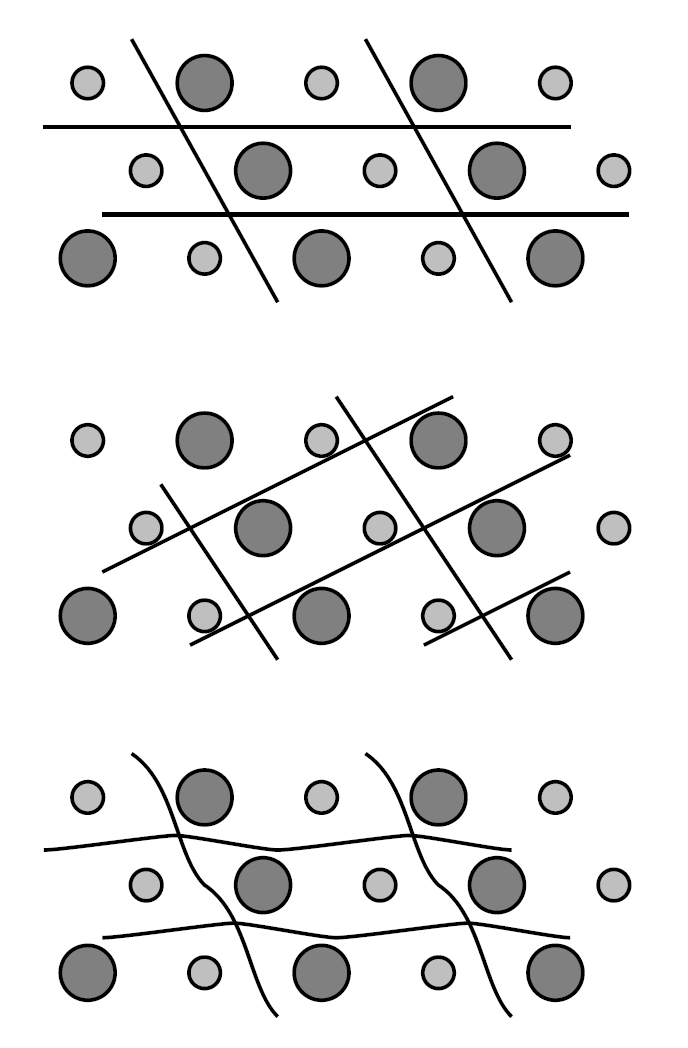
\includegraphics[scale=0.4]{Cuerpo/Ch_01/Celda_unitaria.png}
	\caption{La elección de una celda unitaria no es única. Todas estas celdas unitarias pueden ser usadas para reconstruir el cristal.}
	\label{Fig:01-001}
\end{figure}

\begin{definition}[{\bf Celda unitaria primitiva}]
    Decimos que la red y los vectores son primitivos si dos puntos cualesquiera $\rn$ y $\rn'$ satisfacen siempre la expresión \ref{Ec:01-01-01} con una adecuada selección de los números enteros $u_1,u_2,u_3$. Denominamos como celda al volumen que ocupa dicho punto de red que se puede replicar mediante traslaciones usando vectores primitivos. En el momento que para replicar la estructura se necesita un no entero la celda, aunque se replique, ya no es primitiva. No existe ninguna celda de volumen menor que pueda servir como bloque constructor para la estructura cristalina. Toda celda primitiva es unitaria. La figura \ref{Fig:01-01} muestra en la parte inferior dos posibles celdas unitarias con sus vectores bases asociados.   
\end{definition}

Para una red existe más de una elección de vectores base primitivos. Todas las celdas primitivas tienen el mismo volumen pues tienen asociado uno y sólo un punto de red. Todos los puntos de una red son indistinguibles en el sentido de que la red {\it se ve} igual desde cualquiera de sus puntos (propia definición de red). También se puede decir que es invariante por traslaciones de vectores de red (\textit{simetría de traslación}). 

\begin{definition}[{\bf Vectores base y celdas no primitivas}]
    Vectores base {\bf no primitivos}: son aquellos que generan la red por combinaciones lineales de la forma de la ecuación \ref{Ec:01-01-01} pero donde los $u_i$ toman también valores no enteros. Un ejemplo es la celda cuadrada centrada que se muestra en la figura . Las \textbf{celdas (unitarias) no primitivas} o \textbf{celdas convencionales} correspondientes son siempre de mayor volumen que las primitivas por tener asociado más de un punto de red. Para algunos propósitos (por ejemplo, la {\it indexación} de máximos de difracción de rayos x que se verá en el Capitulo \ref{Ch:02}) la combinación red+base puede variarse, aunque sea a costa de aumentar el número de átomos de la base. En la figura \ref{Fig:01-01} puede verse en la parte superior un conjunto de vectores base que no forman una celda primitiva, mientras en la parte inferior (e inferior izquierda) podemos ver vectores base que sí forman una celda primitiva.
\end{definition}

\begin{definition}[{\bf Celda de Wigner-Seitz}]
Se construye de la siguiente forma: trazar segmentos que concecntan a un punto dado de la red con todos sus vecinos próximos; trazar los planos mediatrices a dichas líneas. La región así encerrada (poliedro en 3D, polígono en 2D) es la celda de Wigner-Seitz. Ver el ejemplo 2D de la Figura \ref{Fig:01-02} . La celda de Wigner-Seitz es \textbf{siempre primitiva} y contiene todas las simetrías de la red.    
\end{definition}


\begin{figure}[h!] \centering
    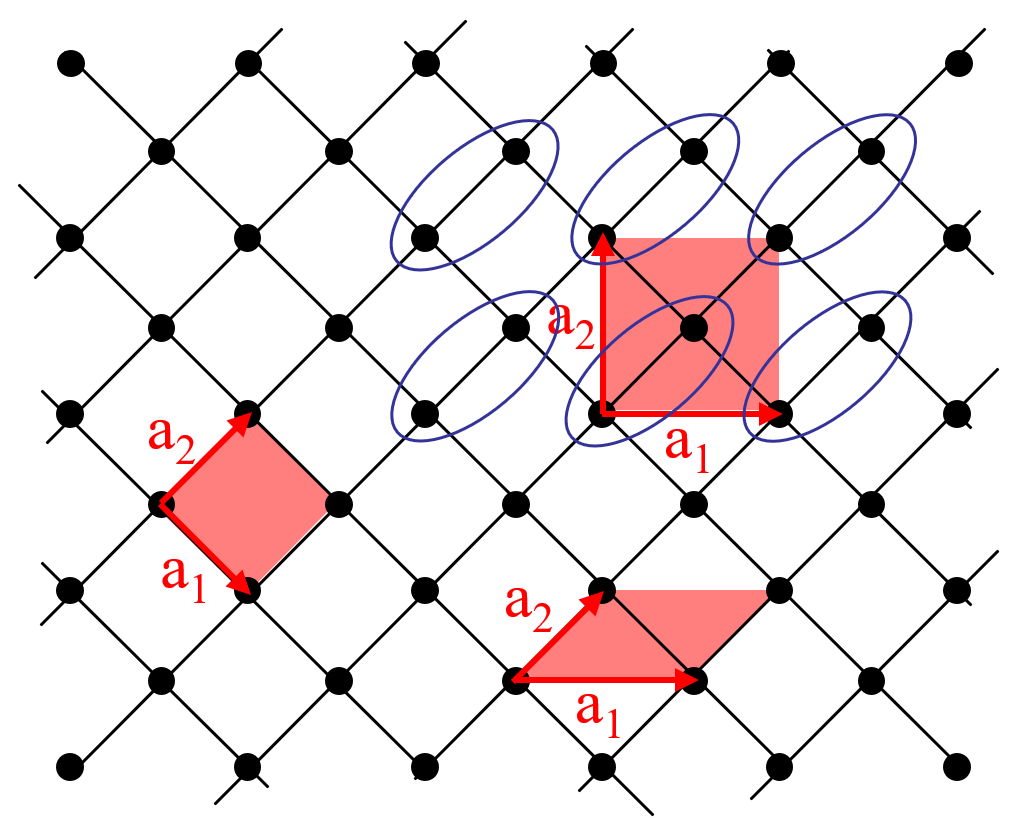
\includegraphics[scale=0.55]{Cuerpo/Ch_01/celda.png}
    \caption{Ejemplos de vectores unitarios y sus correspondientes celdas unitarias.}
    \label{Fig:01-01}
\end{figure}

\begin{figure}[h!] \centering
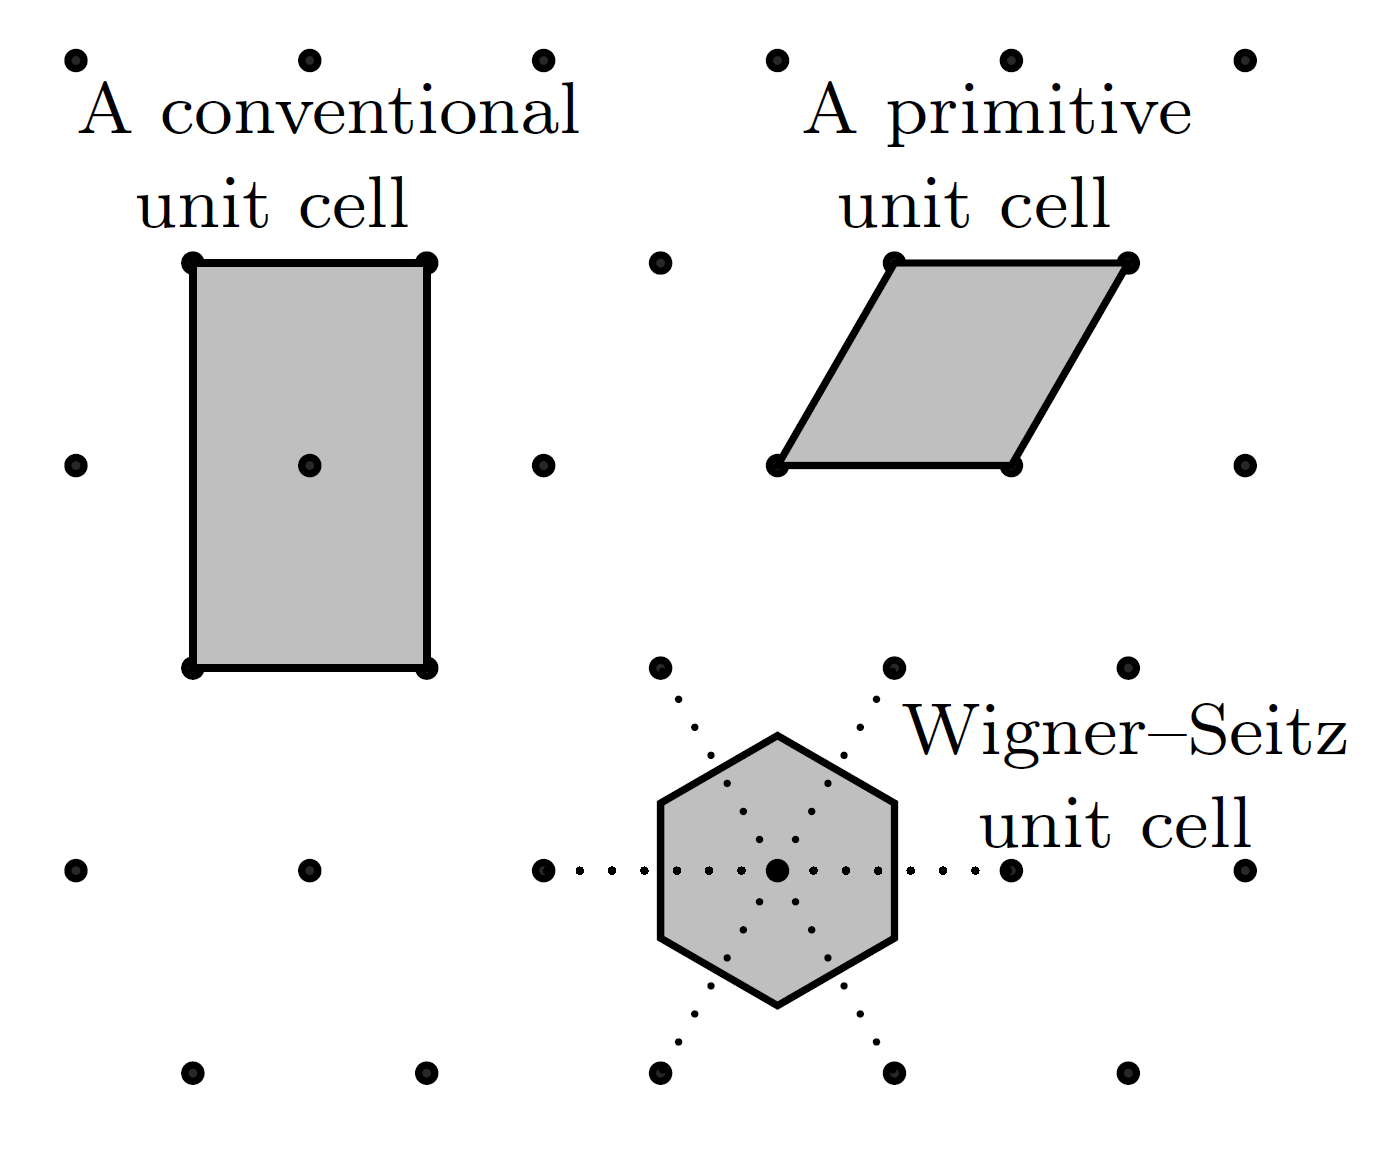
\includegraphics[scale=0.4]{Cuerpo/Ch_01/Celdas.png}
\caption{Podemos ver algunas de las celdas unitarias para una red triangular.}
\label{Fig:01-011}
\end{figure}

\subsection{Otras definiciones}
  
\begin{definition}[{\bf Otras simetrías}]
    Invariancia por {\it inversión} ($\Rn \rightarrow - \Rn$), {\it eje de rotación} de orden $n$ (invariancia por giro del ángulo $2\pi/n$ alrededor del eje), {\it planos de simetría, centros de inversión}...    
\end{definition}

\begin{definition}[{\bf Número de coordinación}]
    Es la número de vecinos más próximos (misma distancia) a un punto cualquiera de la red. La misma noción se aplica a átomos cuando se trata de cristales. También se le llamad \textbf{índice de coordenación} o \textbf{número de primeros vecinos}.
\end{definition}

\begin{definition}[{\bf Familia de planos reticulares}]
    Conjunto de planos paralelos y equiespaciados que contienen todos los puntos de la red. 
\end{definition}


\begin{definition}[{\bf Número de defectos de Schottky}]
    (vacantes) en un cristal a temperatura $T$:
    \begin{equation}
    n \approx N e^{-\epsilon_v /k_B T}
    \end{equation}
    $N$ es el número de átomos y $\epsilon_v$ la energía necesaria para formar una vacante. Se desarrolla mejor en los apartados \ref{Subsec:01-06-01} y \ref{Subsec:01-06-02}.
\end{definition}


\begin{definition}[{\bf Número de defectos de Frenkel}]
    (vacantes-átomos interesticiales) en un cristal a temperatura $T$:
    \begin{equation}
    n \approx \sqrt{NN'} e^{-\epsilon_F /k_B T}
    \end{equation}
    $N$ es el número de átomos , $N'$ en número de intersticios, y $\epsilon_vF$ la energía necesaria para formación de un defecto de este tipo. Se desarrolla mejor en los apartados \ref{Subsec:01-06-01} y \ref{Subsec:01-06-02}.
\end{definition}
    

\begin{figure}[h!] \centering
    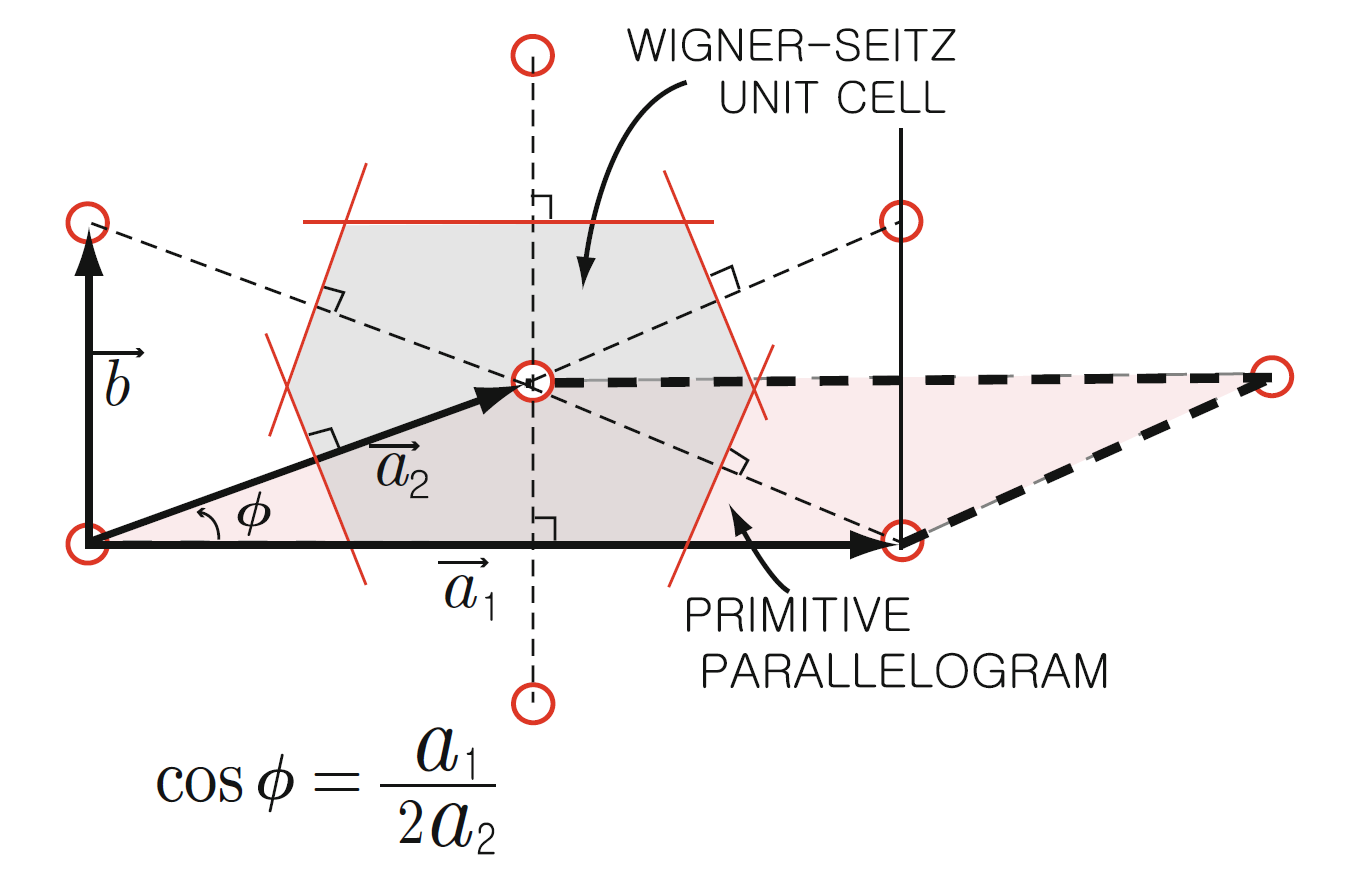
\includegraphics[scale=0.3]{Cuerpo/Ch_01/Wigner-seitz_1.png}
    \caption{celda de Wigner-seitz 2D.}
    \label{Fig:01-02}
\end{figure}



 \section{Tipos fundamentales de redes: Redes de Bravais}

En la figura \ref{Fig:01-03} podemos ver los 14 tipos de redes, llamadas {\bf redes de Bravais}. Solo las celdas etiquetadas como {\it simples} son primitivas. Estos 14 tipos pueden agruparse a su vez en los 7 {\it sistemas cristalinos} indicados en la  tabla \ref{Tab:01-01} (cuando escribimos $a=b=c$ (o $a_1=a_2=a_3$) nos referimos a que todos los lados son igual de largos).

\begin{table}[h!] \centering
    \begin{tabular}{cccc}
        Sistema  & Simetría  & Número de & Características de \\ 
        cristalino & característica & redes de Bravais & la celda unitaria \\
        \hline \hline 
        Triclínico & Ninguna & 1 (Simple) & $a \neq b \neq c$ \\
        & & & $\alpha \neq \beta \neq \gamma \neq 90^o$ \\ \hline
        Monoclínico & 1 eje de rotación & 2 (Simple, centrada & $a \neq b \neq c$ \\
        & binario (n=2) & en las bases) & $\alpha = \beta = 90^o \neq \gamma$ \\ \hline Ortorrómbico & 2 ejes binarios & 4 (Simple, Centrada & $a \neq b \neq c$ \\
        & (n=2) mutuamente & en las bases, Centrada & $ \alpha = \beta = \gamma = 90^o$ \\
        & perpendiculares & en el cuerpo, Centrada & \\
        & & en las caras) & \\ \hline
        Tetragonal  & 1 eje cuaternario & 2 (Simple, Centrada & $a=b\neq c$ \\
        & (n=4) & centrada en el cuerpo) & $ \alpha = \beta = \gamma = 90^o$ \\ \hline
        Cúbico & 4 ejes cuaternarios & 3 (Simple, Centrada & $a=b=c$ \\
        & (n=4) perpendiculares & en el cuerpo, Centrada & $ \alpha = \beta = \gamma = 90^o$ \\ 
        & entre sí & en las caras)  & \\ \hline 
        Hexagonal & 1 eje senario & 1 (Simple) & $a=b\neq c$ \\
        & (n=6) & & $\alpha=120^o$  \\
        & & & $\beta = \gamma = 90^o$ \\ \hline
        Romboédrica& 1 eje ternario & 1 (Simple) & $a=b=c$ \\ 
        & (n=3) & & $120^o > \alpha = \beta = \gamma \neq 90^o$\\ \hline
    \end{tabular}
    \caption{Redes de Bravais en función del sistema cristalino.}
    \label{Tab:01-01}
\end{table}


\begin{figure}[h!] \centering
    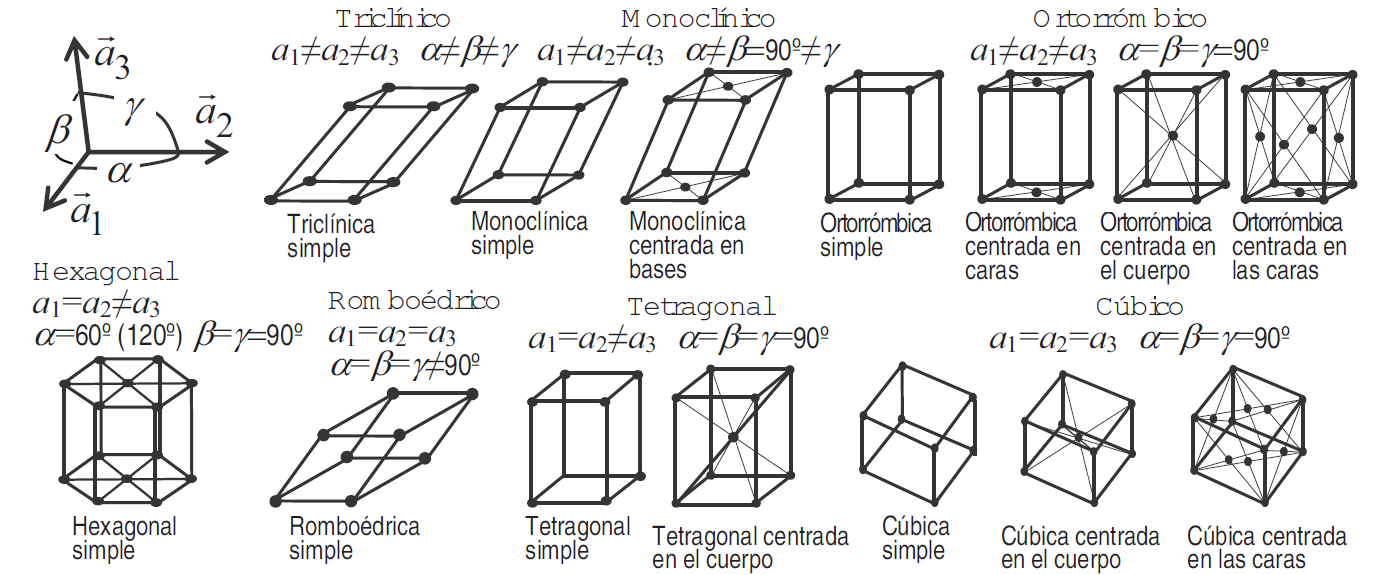
\includegraphics[scale=0.73]{Cuerpo/Ch_01/Redes_bravais.png}
    \caption{celdas unitarias de las 14 posibles redes de Bravais.}
    \label{Fig:01-03}
\end{figure}

\subsection{Características de las redes del sistema cúbico}

Las redes del sistema cúbico son las redes mas importantes, por tanto conocer sus características (vectores base primitivo, número de primeros y segundos vecinos, distancias entre vecinos...) es fundamental. Por eso presentamos la tabla \ref{Tab:01-03}, para tener una referencia a la hora de hacer ejercicios. Como siempre la elección de los vectores unitarios primitivos es arbitraria, siempre habiendo otra posible elección. Por ejemplo otro vector base para la \bcc (de hecho es la escogida en el \cite{Oxford_Solid_State}) puede ser

\begin{equation}
	\an_1 = (1,0,0) \quad \an_2 = (0,1,0) \quad \an_3 = (1/2,1/2,1/2) 
\end{equation}

\begin{table}[h!] \centering
	\begin{tabular}{lccc}
		Red (parámetro $a$) & \sc & \bcc & \fcc \\ \hline 
		& $\an_1=a\hni$ &  $\an_1=a\hni$ & $\an_1=a\hni$  \\		
		Vectores unitarios por celda convencional  & $\an_2=a\hnj$  & $\an_2=a\hnj$  &  $\an_2=a\hnj$ \\
		& $\an_3=a\hnk$ & $\an_3=a\hnk$  & $\an_3=a\hnk$ \\ \hline
		Volumen celda convencional & $a^3$ & $a^3$ & $a^3$ \\ \hline
		Puntos de red por celda convencional & 1 & 2 & 4 \\ \hline
		Puntos de red por unidad de volumen & $1/a^3$ &  $2/a^3$ &  $4/a^3$ \\ \hline
		Número de vecinos más próximos & $a$ & $a\sqrt{3}/2$ & $a/\sqrt{2}$ \\ \hline
		Distancia entre vecinos más próximos & $a$ & $a\sqrt{3}/2$ & $a/\sqrt{2}$ \\ \hline
		Número de segundos vecinos & 12 & 6 & 6 \\ \hline
		Distancia entre segundos vecinos & $\sqrt{2} a$ & $a$ & $a$ \\ \hline
		& $\an_1=a\hni$ &  $\an_1=\frac{1}{2} a (-\hni+\hnj+\hnk)$ &   $\an_1=\frac{1}{2} a (\hnj+\hnk)$  \\
		Vectores unitarios primitivos &$\an_2=a\hnj$ &  $\an_2=\frac{1}{2} a (\hni-\hnj+\hnk)$ &   $\an_2=\frac{1}{2} a (\hni+\hnk)$  \\
		&$\an_3=a\hnk$ &  $\an_3=\frac{1}{2} a (\hni+\hnj-\hnk)$ &   $\an_3=\frac{1}{2} a (\hni+\hnj)$  \\ \hline		
	\end{tabular}
	\caption{Características de las redes del sistema cúbico}
	\label{Tab:01-03}
\end{table} 

\begin{figure}[h!] \centering
	\begin{subfigure}[b]{0.45\linewidth} \centering
	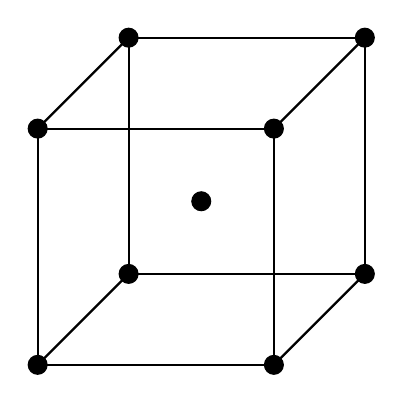
\begin{tikzpicture}[scale=3]% Dibujar los vértices del cubo
		\foreach \x in {0,1} {
			\foreach \y in {0,1} {
				\foreach \z in {0,1} {
					\filldraw (\x,\y,\z) circle (0.04); % Átomos en los vértices
				}
			}
		}
		
		% Dibujar el átomo en el centro del cubo
		\filldraw (0.5,0.5,0.5) circle (0.04); % Átomo en el centro del cubo
				% Aristas del cubo
		\draw[thick] (0,0,0) -- (1,0,0);
		\draw[thick] (0,0,0) -- (0,1,0);
		\draw[thick] (0,0,0) -- (0,0,1);
		\draw[thick] (1,0,0) -- (1,1,0);
		\draw[thick] (1,0,0) -- (1,0,1);
		\draw[thick] (0,1,0) -- (1,1,0);
		\draw[thick] (0,1,0) -- (0,1,1);
		\draw[thick] (0,0,1) -- (1,0,1);
		\draw[thick] (0,0,1) -- (0,1,1);
		\draw[thick] (1,1,0) -- (1,1,1);
		\draw[thick] (1,0,1) -- (1,1,1);
		\draw[thick] (0,1,1) -- (1,1,1);
		
	\end{tikzpicture}
	\caption{\bcc.}
	\end{subfigure}
	\begin{subfigure}[b]{0.45\linewidth}	\centering		
			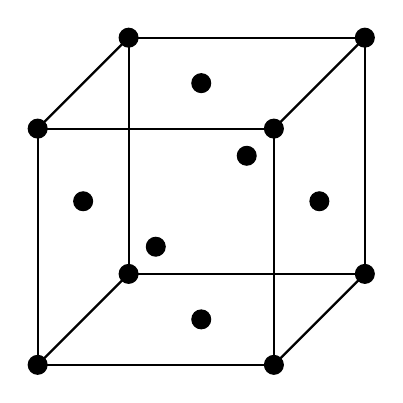
\begin{tikzpicture}[scale=3]
				
				% Dibujar los vértices del cubo
				\foreach \x in {0,1} {
					\foreach \y in {0,1} {
						\foreach \z in {0,1} {
							\filldraw (\x,\y,\z) circle (0.04); % Átomos en los vértices
						}
					}
				}
				
				% Dibujar los átomos en el centro de las caras
				\filldraw (0.5,0.5,0) circle (0.04); % Cara xy abajo
				\filldraw (0.5,0.5,1) circle (0.04); % Cara xy arriba
				\filldraw (0.5,0,0.5) circle (0.04); % Cara xz izquierda
				\filldraw (0.5,1,0.5) circle (0.04); % Cara xz derecha
				\filldraw (0,0.5,0.5) circle (0.04); % Cara yz delante
				\filldraw (1,0.5,0.5) circle (0.04); % Cara yz detrás
				
				% Etiquetas de los ejes
			%	\draw[->] (-0.2,0,0) -- (1.3,0,0) node[anchor=north east] {$x$};
			%	\draw[->] (0,-0.2,0) -- (0,1.3,0) node[anchor=north west] {$y$};
			%	\draw[->] (0,0,-0.2) -- (0,0,1.3) node[anchor=south] {$z$};
				
				% Aristas del cubo
				\draw[thick] (0,0,0) -- (1,0,0);
				\draw[thick] (0,0,0) -- (0,1,0);
				\draw[thick] (0,0,0) -- (0,0,1);
				\draw[thick] (1,0,0) -- (1,1,0);
				\draw[thick] (1,0,0) -- (1,0,1);
				\draw[thick] (0,1,0) -- (1,1,0);
				\draw[thick] (0,1,0) -- (0,1,1);
				\draw[thick] (0,0,1) -- (1,0,1);
				\draw[thick] (0,0,1) -- (0,1,1);
				\draw[thick] (1,1,0) -- (1,1,1);
				\draw[thick] (1,0,1) -- (1,1,1);
				\draw[thick] (0,1,1) -- (1,1,1);
				
			\end{tikzpicture}
			\caption{\fcc.}
	\end{subfigure}
	\caption{Imagenes de las celdas convencionales de la fcc y la bcc}
\end{figure}

\subsection{Red diamante}

La red diamante tampoco es mencionada en el \cite{Fisica_del_Estado_Solido} pero sí en el \cite{Fisica_del_Estado_Solido_Resueltos}, por lo que es importante describirla, aunque sea escuetamente, para poder hacer algún ejercicio. La \textbf{red diamante} es una red \fcc \ pero con una base diatómica, de tal modo que si uno de los átomos está en $\rn$ el otro se encontrará en $\rn+a(1/4,1/4,1/4)$. 

Las características de la red diamante son las mismas que la fcc pero teniendo en cuenta la base diatómica, por lo que el número de puntos de red para la celda convencional es 4 pero el número de átomos será 8. Por otro lado cambiará el número de primeros vecinos (ahora son 4, ya que cada átomo esta en un tetraedro), mientras que la fracción de empaquetamiento es del 34\%. El ángulo entre los vectores que unen dos primeros vecinos con un átomo es de 108$^o$47', lo cual se peude calcular usando el producto escalar.



\section{Empaquetamiento compacto}

Una pregunta interesante es la de cuáles son las estructuras (cristalinas) más compactas que se pueden construir con esferas iguales. Primero se formaría una capa A de máxima compacidad en la que la que cada esfera está en contacto con otras seis (círculos continuos de la figura \ref{Fig:01-04}, parte superior). Una segunda capa B idéntica se situaría encima de la primera, ocupando la mitad de los huecos intersticiales de la capa A. Una tercera capa se puede añadir de dos maneras: sobre los huecos de la primera capa no ocupados por la segunda, dando lugar ala secuencia ABCABC..., o sobre la vertical de las esferas de la primera capa generando la secuencia ABABAB...

\begin{figure}[h!] \centering
    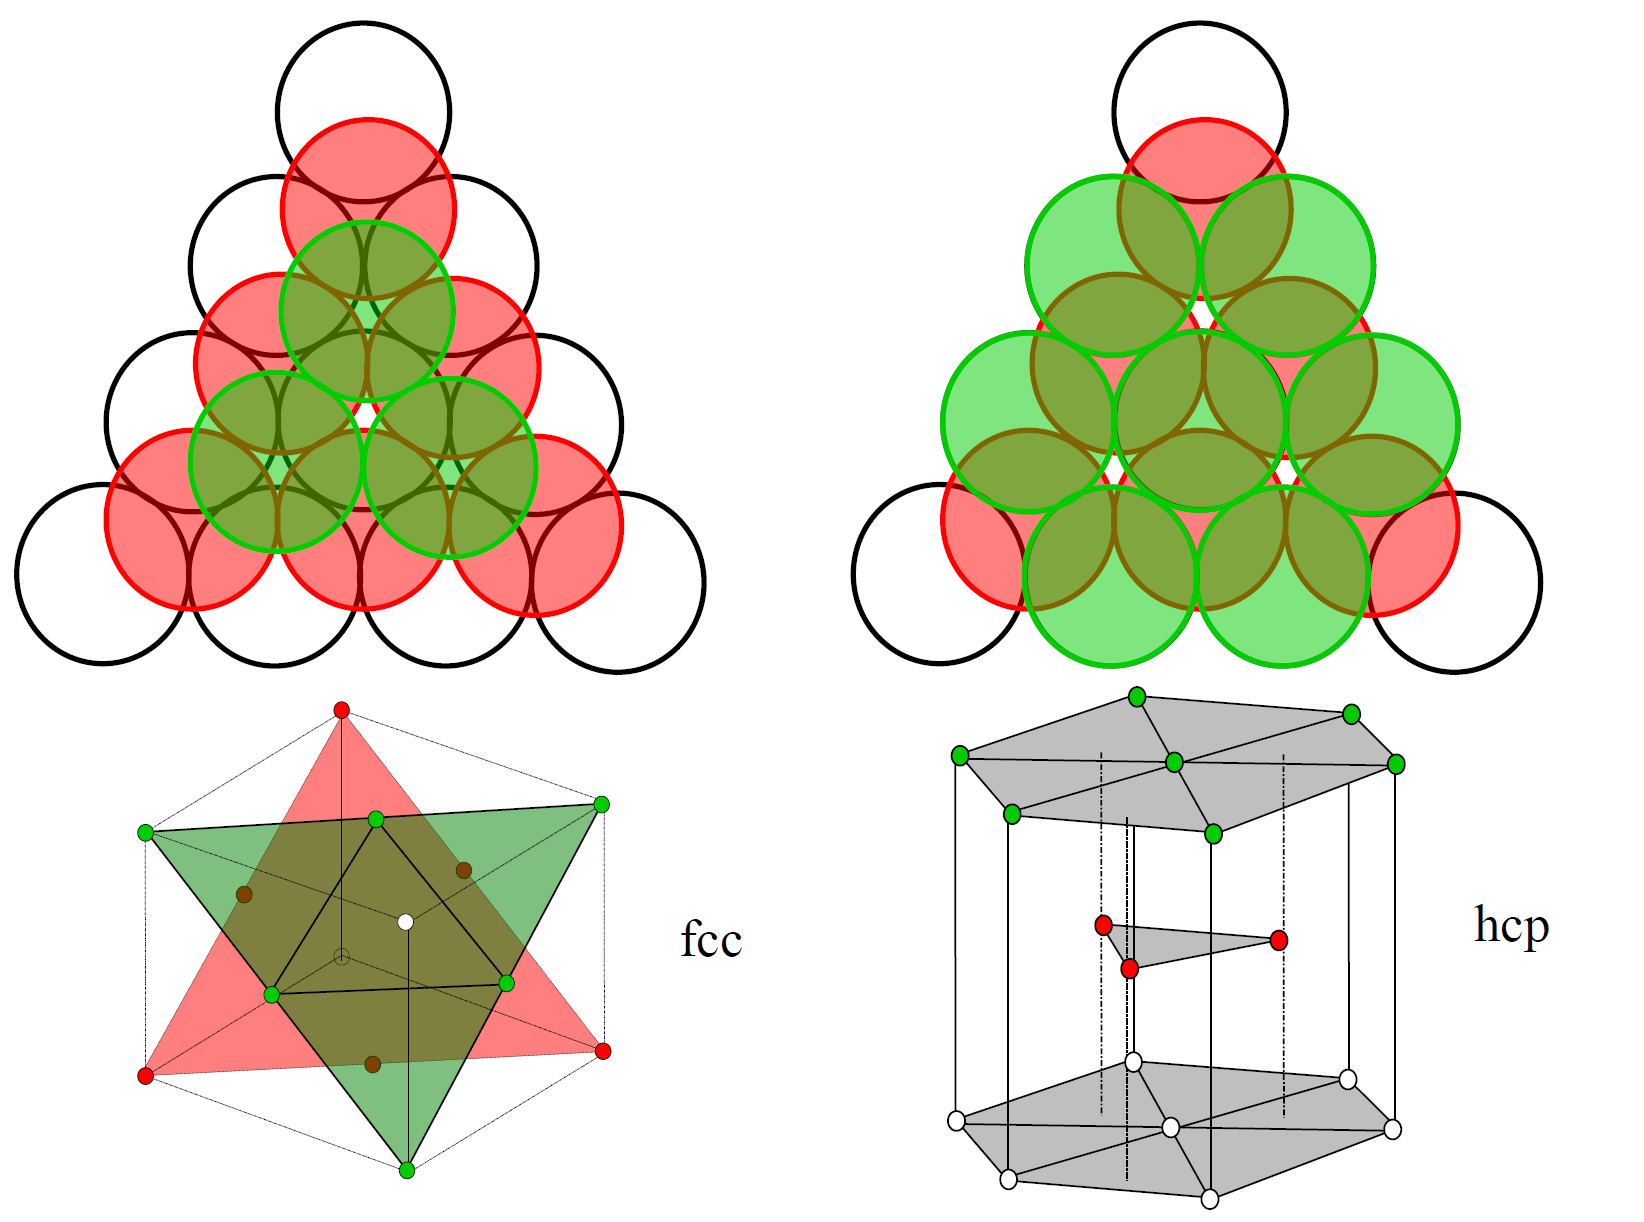
\includegraphics[scale=0.2]{Cuerpo/Ch_01/Empaquetamiento_compacto.png}
    \caption{Empaquetamiento compacto.}
    \label{Fig:01-04}
\end{figure}

En el primer caso la estructura resultante es una {\it fcc}, donde las capas de que hablamos son las perpendiculares a la diagonal del cubo (figura \ref{Fig:01-04}, parte inferior izquierda). En el segundo caso las capas A,B se corresponden con los planos basal e intercalado, respectivamente, de una estructura diagonal compacta ({\it hcp}) (figura \ref{Fig:01-04} parte inferior derecha). Se describe como un red hexagonal (capas A) con una base dos átomos (capas B). En ambas estructuras el número de coordinación es 12. 

\begin{definition}[\textbf{fracción de empaquetamiento}] Definimos la fracción de empaquetamiento (f.e.) como la cantidad de espacio ocupada por los átomos (suponiendo que son esféricos, de radio $r$) en la celda convencional y el volumen de la celda convencional (también se puede ser usada otra celda, pero por comodidad se usa esta).	
\end{definition}
Las fracciones de empaquetamiento para algunas de las estructuras más comunes son: 

\begin{table}[h!] \centering
	\begin{tabular}{c|c|c|c|c}
	 &	\sc  & \bcc & \fcc & Hexagonal compacta \\ \hline \vspace{0.5cm}
	 f.e. & $\frac{\pi}{6} \approx 52\%$ & $\frac{\pi \sqrt{3}}{8} \approx 68\%$ & $\frac{\pi \sqrt{2}}{6} \approx 74\%$ & $\frac{\pi \sqrt{2}}{6} \approx 74\%$ 
	\end{tabular}
	\caption{fracciones de empaquetamiento compacto para algunas estructuras.}
\end{table}


\section{Intersticios o huecos estructurales}

Muchos compuestos cristalinos se pueden entender mejor si se conocen los huecos estructurales (entendiendo esto por las mayores oquedades o intersticios entre átomos) asociados a las estructuras básicas. Ilustraremos esto con las redes del sistema cúbico. Ilustraremos esto con la figura \ref{Fig:01-05}.

En la red \textit{fcc} los mayores huecos son octaédricos, de radio $0.41$R. Hay tantos huevos octaédricos como átomos, situándose en los centros de los cubos y de las aristas. Hay también huecos tetraédricos de radio 0.22R. Hay el doble de número de huecos tetraédricos que de átomos. Así, el NaCl es descriptible como una {\it fcc} de iones Cl$^-$ en cuyos intersticios octaédricos se sitúan los iones de Na$^+$. También el diamante o la blenda de cinc se pueden considerar como una estructura {\it fcc} (de C ó S) en la que la mitad de los huecos tetraédricos están ocupados por los átomos de C o de Zn, respectivamente. En la \bcc  los huecos más grandes son los tetaédricos, aunque también son los más difíciles de visualizar (véase imágenes inferiores de la figura \ref{Fig:01-05}).

En la red {\it bcc} existen 6 huevos octaédricos (distorsionados) por celda, situados en los centros de las caras y de las aristas. Sin embargo, los mayores intersticios se dan en los 12 tetaédricos (también distorsionados) por celda: su radio es 0.29R. Como un ejemplo de aplicación, digamos que la gran movilidad de los iones Ag$^+$ en el AgI, un excelente elcetrólito sólido usado en pilas de estado sólido, proviene de que los 2 iones Ag$^+$ por celda se distribuyen estadísticamente entre las 12 posiciones tetraédricas de la red {\it bcc} que forman los iones I$^-$ saltando fácilmente de unas a otras.


\begin{figure}[h!] \centering
    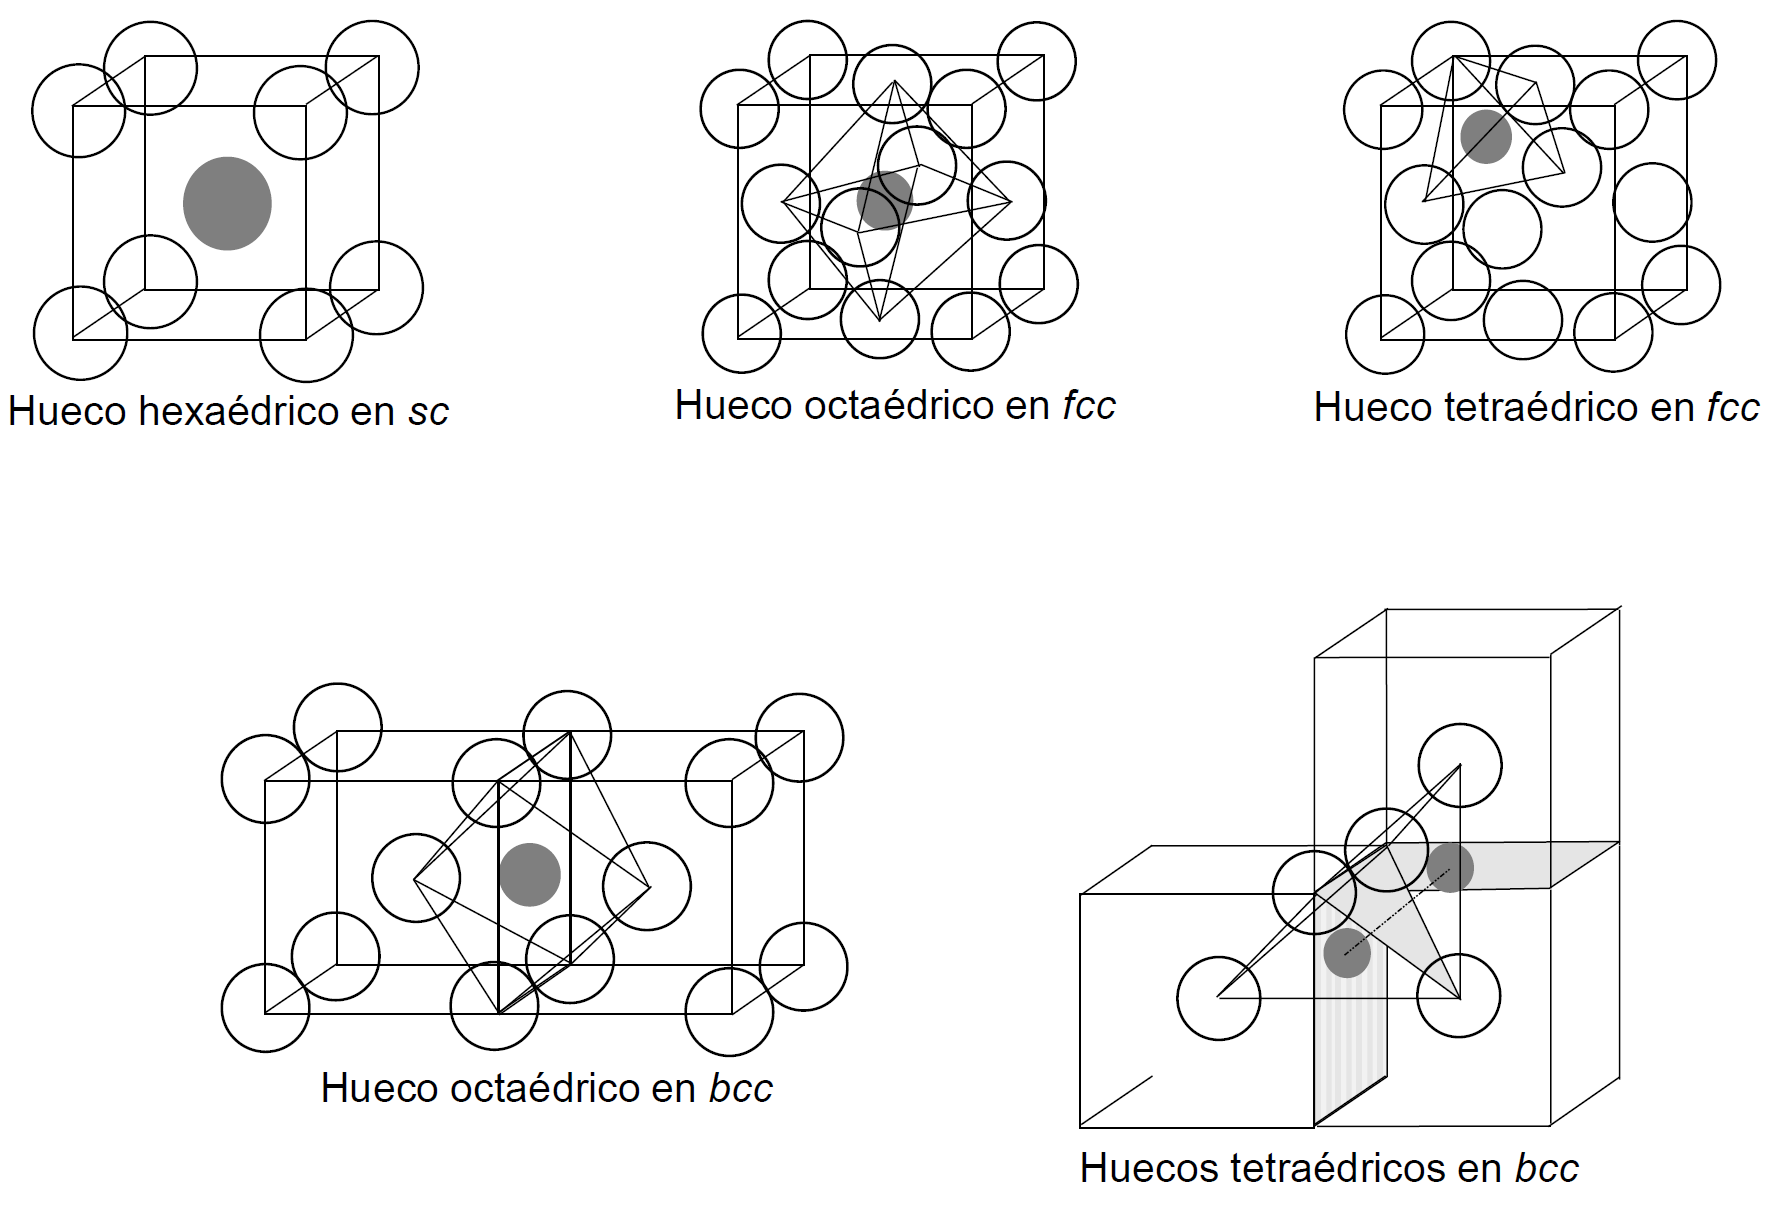
\includegraphics[scale=0.4]{Cuerpo/Ch_01/huecos.png}
    \caption{Localización de algunos huecos.}
    \label{Fig:01-05}
\end{figure}


\section{Defectos y desorden en los cristales}

El cristal perfecto tal como se ha introducido no existe, sino que posee varias clases de imperfecciones o defectos que suelen clasificarse en cuatro clases atendiendo a su dimensión, es decir, su número de dimensiones espaciales en las cuales las alteraciones de la estructura se extienden a distancias (mucho) mayores que el parámetro de red, tal y como se indica en la tabla.


\begin{table}[h!] \centering
    \begin{tabular}{m{2cm} | m{4cm} | m{4cm} | m{4cm}}
        Defecto & Descripción & Ejemplos & Origen \\ \hline \hline
        Puntual & Alteración localizada en puntos aislados del cristal. Su extensión no supera en ninguna dirección más de una o unas pocas veces el parámetro de red. & - Vacantes \newline - Átomos intersticiales \newline -Impurezas sustitucionales/intersticiales \newline -Huecos dobles, triples, etc. & -Térmico \newline -Irradiación \newline -Desviaciones de la estequiometría \newline -Deformación plástica \\ \hline
        Lineal & Alteración en 1 dirección muchas veces el parámetro de red & -Dislocaciones \newline -Cadenas de defectos puntuales & - Proceso de crecimiento \newline -Deformación plástica \\ \hline
        Superficial & Alteración en 2 direcciones muchas veces el parámetro de red & -Bordes de granos \newline -Maclas \newline Superficies del cristal & -Proceso de crecimiento \newline -Deformación plástica \newline -Impurezas en la masa fundida \\ \hline
        Espacial & Alteración en las 3 direcciones muchas veces el parámetro de red & -Poros \newline -Inclusiones de otra fase & Ídem \\ \hline
    \end{tabular}
    \caption{Clasificación de los principales defectos en cristales.}
    \label{Tab:01-02}
\end{table}





\subsection{Defectos puntuales} \label{Subsec:01-06-01}

El defecto puntual más simple es la vacante: ausencia de un átomo en su posición de la red (defecto de Schottky). Se forman cuando, debido a la agitación térmica, algunos átomos de la capa más próxima a la superficie saltan a ésta. Este hueco emigra por el interior del cristal pues se necesita poca energía para que un átomo vecino se mueva a una vacante, dejando su propio sitio vacío. Los cristales iónicos, donde las vacantes se forman a pares para mantener la neutralidad eléctrico, deben su débil conductividad $[ \sigma \approx 10^{-6} (\Omega m)^{-1} \ vs \ 10^8 (\Omega m)^{-1}$ de los metales] a esta movilidad de sus  átomos. Otro tipo de defecto puntual (térmico) es el defecto de Frenkel, que es un átomo que ha abandonado el nudo de la red y que se aloja en un intersticio. Se trata en realidad de la combinación de una vacante y un átomo intersticial. % ahora habla de una figura

Los defectos de Schottky o las impurezas sustitucionales se encuentran de ordinario en los cristales de empaquetamiento denso ({\it fcc} o {\it hcp}), en los cuales el alojamiento de átomos en los intersticios es difícil, mientras que los defectos de Frenkel o las impurezas intersticiales suelen formarse en los cristales de empaquetamiento menos denso (diamante), aunque, en el caos de la adición de impurezas, el tipo de defecto que se forme depende del tamaño del átomo de impureza. Por ejemplo, cuando se carburiza hierro ({\it bcc}), el carbono, por su pequeño tamaño, se difunde hacia el interior intesrsticialmente. En cambio, las impurezas con que se dopan los semiconductores (diamante) se sitúan en las posiciones regulares. Otro ejemplo son las aleaciones. Así, el bronce no es sino el Cu metálico en el que una pequeña proporción de sus átomos ha sido sustituida por átomos de Sn, constituyendo una solución sólida. 

\begin{figure}[h!] \centering
    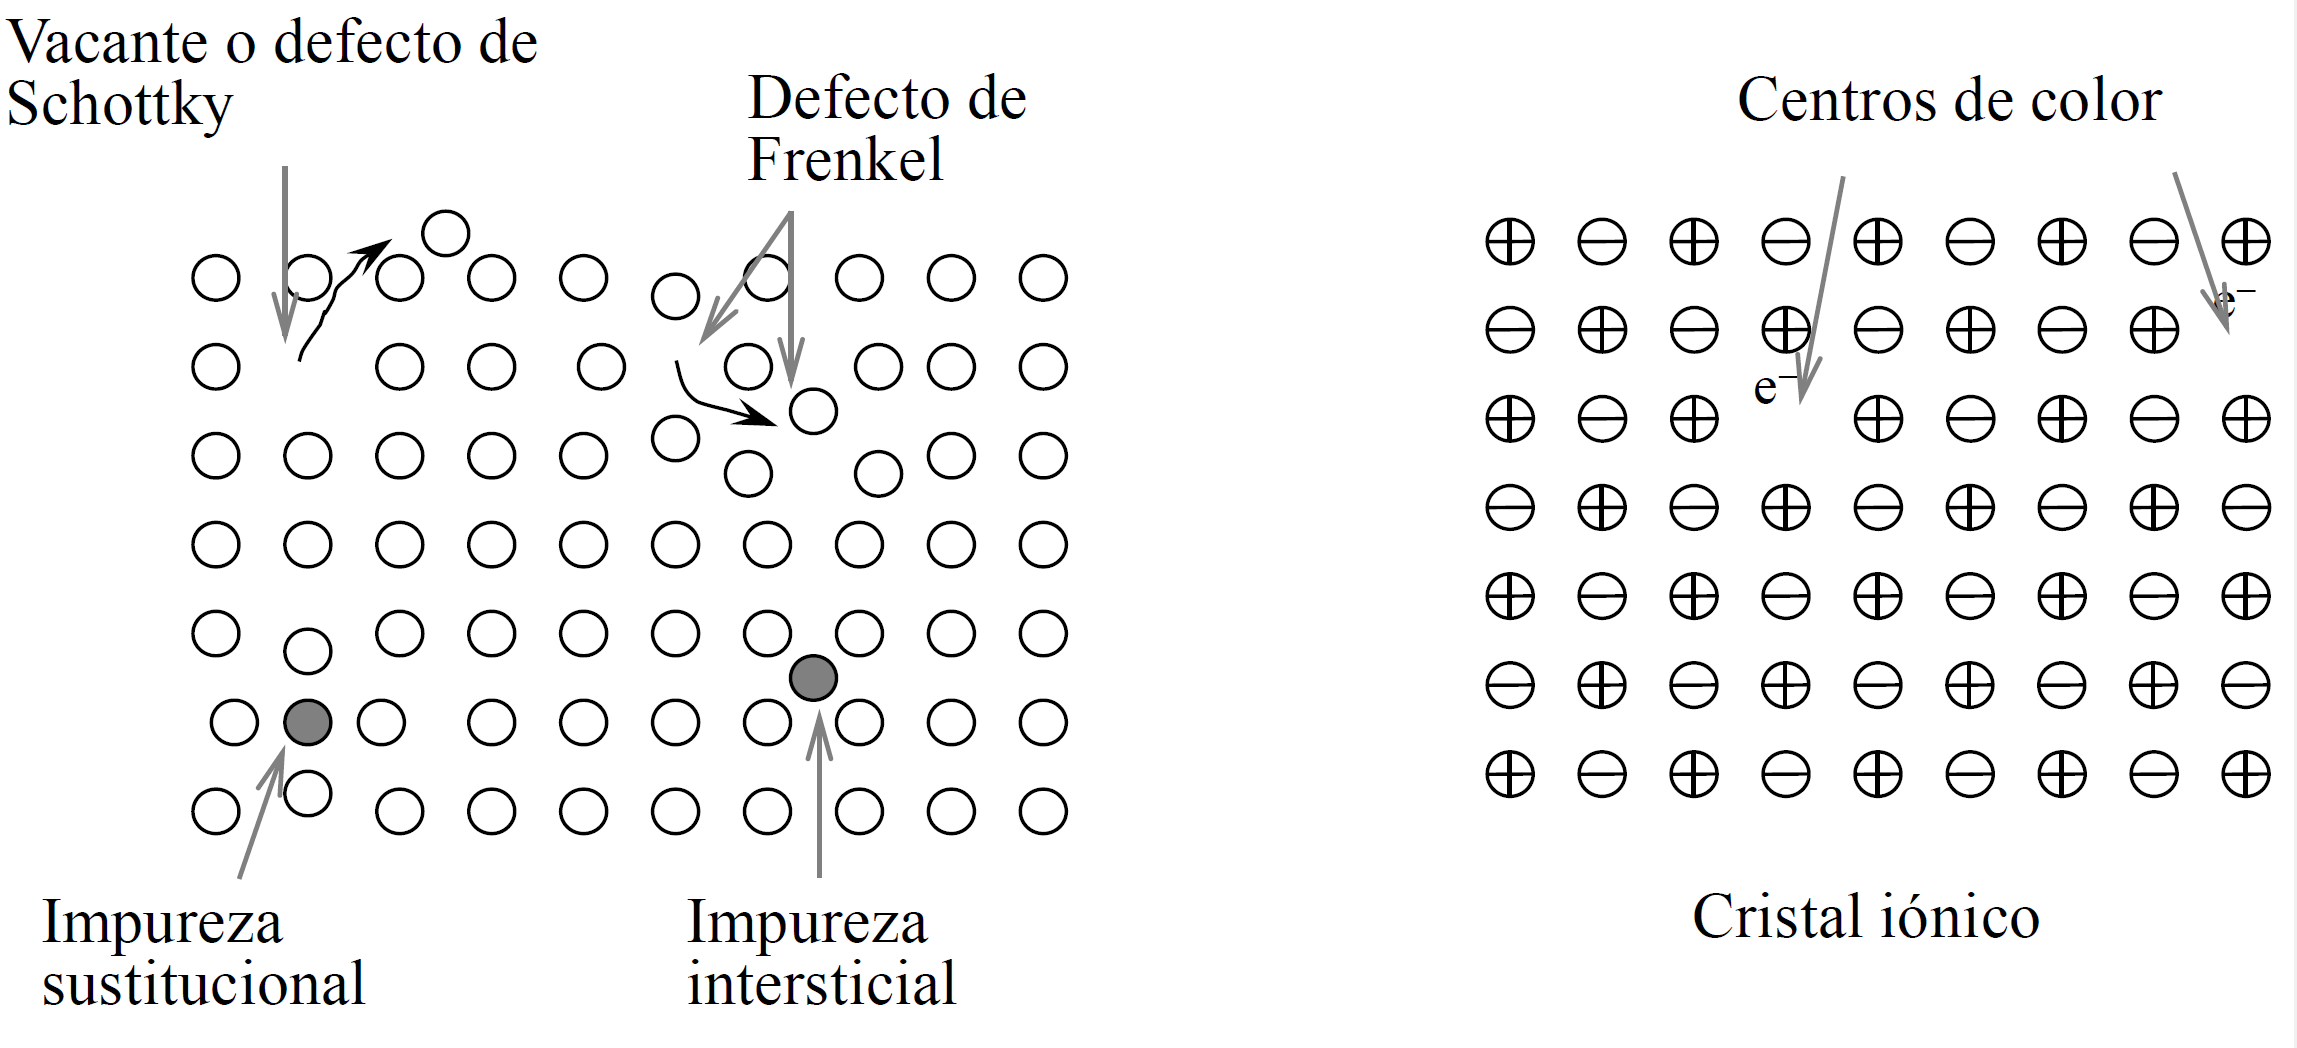
\includegraphics[scale=0.42]{Cuerpo/Ch_01/defectos.png}
    \caption{Defectos puntuales.}
\end{figure}


En los cristales iónicos también los electrones pueden participar en la formación de defectos, como los llamados {\it centro de color} (en los haluros alcalinos, por ejemplo), donde un hueco aniónico (ausencia de un ion negativo) atrapa a un electrón libre. El electrón, así atrapado, tiene une espectro de niveles similar al de los niveles atómicos. Así, este centro F hace que aparezca una banda de absorción en la {\it región visible} del espectro. A esto se debe que un cristal de haluro alcalino incoloro se coloree cuando se fuerza la aparición de huecos aniónicos por irradiación con rayos $x$ o $\gamma$.


\subsection{Concentración de defectos térmicos puntuales en equilibrio} \label{Subsec:01-06-02}

La formación de defectos puntuales requiere un aporte de energía al cristal proporcional a al energía de enlace (así, por ejemplo, la energía de formación de un hueco es el Ge es $\sim 2$ eV). Sin embargo, a temperaturas relativamente altas resulta energéticamente rentable la existencia de defectos. Esto se debe a que la formación de defectos puntuales no sólo aumenta la energía interna, $E$, del cristal, sino que también aumenta su entropía, $S$, de forma que a una temperatura $R$ la energía libre, $F=E-TS$, es mínima para una cierta concentración, $n$, de defectos. 

Supóngase que hay un sólo tipo de defectos, por ejemplo de Schottky. Si $\epsilon_v$ es la energía para formar una vacante, la necesaria para formar $n$, aisladas y no interaccionantes, será $n\epsilon_v$. La entropía (de configuración) es $S=k_B \ln \Gamma$, donde $\Gamma$ es el número de microestados compatibles con el macroestado, en este caso, simplemente el número de maneras en que $n$ vacantes pueden disponer entre $N$ nudos. Así:

\begin{equation}
    S = k_B \ln \frac{N!}{(N-n)! n!}
\end{equation}
Usando la fórmula de Stirling: $\ln x! \approx x(\ln x - 1)$, para $x\gg 1$, la energía libre se escribe

\begin{equation}
    F = n \epsilon_v - k_B T [N \ln N - (N-n) \ln (N-n) - n \ln n]
\end{equation}
En equilibrio térmico, $(\partial F / \partial n)_T = 0 \Rightarrow \epsilon_v = k_B T \ln [(N-n)/n]$, que para $n\ll  N$ permite despejar

\begin{equation}
    n \approx N e^{-\epsilon_v /k_B T}
\end{equation}
Como ejemplo numérico, para $T=1000$K y $\epsilon_v  \approx $ 1 eV se tiene que $n/N \approx 10^{-5}$. Análogamente, se tratan los defectos de Frenkel. En este caso hay que considerar no sólo las posibilidades de disponer de $n$ vacantes entre $N$ nudos, sino también las posibilidades para disponer de $n$ átomos entre $N'$ intersticios $\Gamma = \frac{N!}{(N-n)! n!}\frac{N'!}{(N'-n)! n!}$. Por lo que el número de defectos en el equilibrio en este caso es:

\begin{equation}
    n \approx \sqrt{NN'} e^{-\epsilon_F / k_B T}
\end{equation}
donde $\epsilon_F$ es la energía necesaria para la formación de un defecto de Frenkel.

\subsection{Defectos de línea}

En la figura \ref{Fig:01-07} se representan un ejemplo del llamado defecto lineal. Se trata de una dislocación en arista, también llamada dislocación de borde y de una dislocación helicoidal. La dislocación de borde se ha producido como resultado del desplazamiento en una distancia atómica de una parte del cristal, la derecha con respecto al plano OMN, mientras que la mitad izquierda permanece inmóvil. Como se puede ver, a $p$ planos atómicos situados debajo del plano de desplazamiento corresponden $p+1$ palmos por encima de dicho plano. El límite dentro la región que ha deslizado y la inmóvil se llama línea de dislocación. Cerca de ésta el cristal está muy deformado. Todo ocurre como si se hubiera removido del cristal un semiplano que termina en la línea de dislocación (también puede pensarse que se añade un semiplano extra). Convencionalmente, la dislocación en arista se designa por el símbolo $\bot$, que apunta hacia el semiplano extra. 

\begin{figure}[h!] \centering
    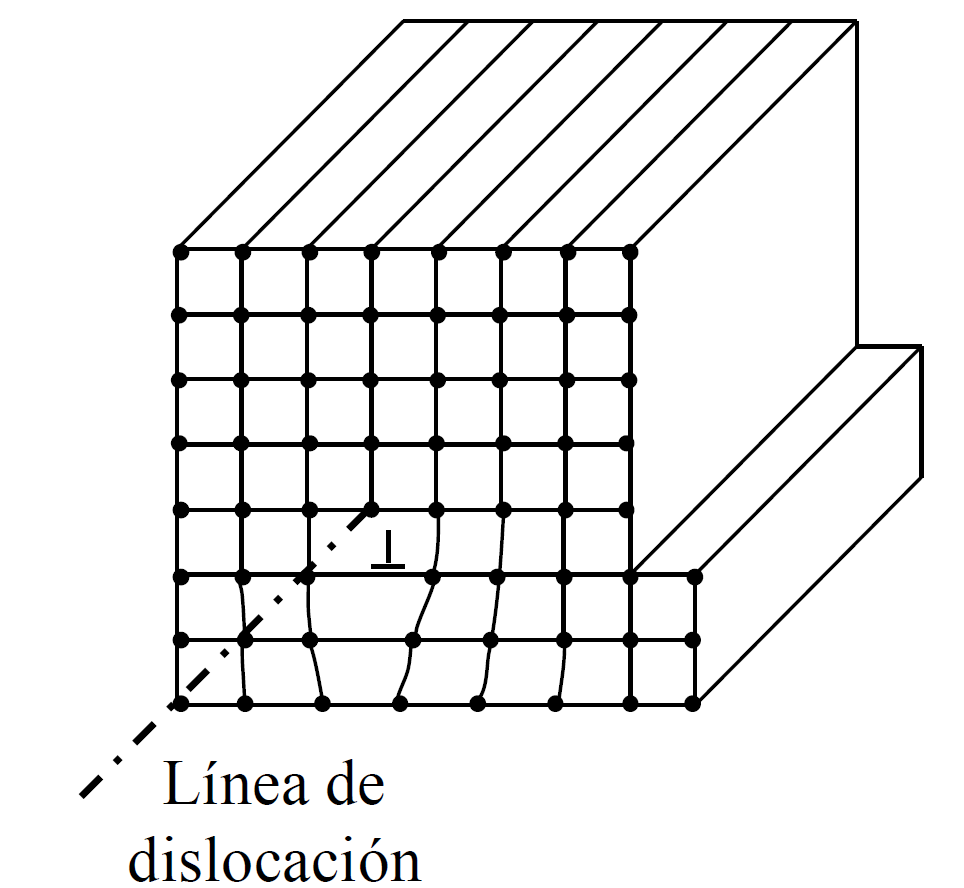
\includegraphics[scale=0.5]{Cuerpo/Ch_01/linea_dislocacion.png}
    \caption{Defectos de línea: línea de dislocación.}
    \label{Fig:01-07}
\end{figure}

Existe una importante relación entre dislocaciones y ciertas propiedades mecánicas como la deformación plástica, que aquí solo se tratan someramente. Por ejemplo, en la figura \ref{Fig:01-08}, para trasladar la dislocación de un extremo a otro solo se requiere un desplazamiento insignificante de los átomos. Una analogía es la arruga en una alfombra: la arruga se mueve más fácilmente que toda la alfombra. De esta forma se puede calcular que valores muy bajos de las tensiones aplicadas a un cristal son suficientes para iniciar una deformación plástica, como en efecto se observa experimentalmente.

\begin{figure}[h!] \centering
    \includegraphics[scale=0.7]{Cuerpo/Ch_01/desplazamiento.png}
    \caption{Desplazamiento de una dislocación bajo fuerza de cizalla.}
    \label{Fig:01-08}
\end{figure}

